\documentclass[conference]{IEEEtran}
% \IEEEoverridecommandlockouts
% The preceding line is only needed to identify funding in the first footnote. If that is unneeded, please comment it out.
\usepackage{amsmath,amssymb,amsfonts}
\usepackage{algorithmic}
\usepackage{graphicx}
\usepackage{textcomp}
\usepackage{xcolor}
\usepackage[backend=biber]{biblatex}

\addbibresource{references.bib}

\usepackage[T1]{fontenc}
\usepackage[utf8]{inputenc}
\usepackage[portuguese]{babel}

\renewcommand\IEEEkeywordsname{Palavras-Chave}

\begin{document}

\title{Análise Estatística sobre Pandemia COVID-19}

\author{\IEEEauthorblockN{Diogo Leite de Pinho Oliveira}
\IEEEauthorblockA{\textit{Departemento de Informática} \\
\textit{ISEP}\\6
Porto, Portugal \\
1181184@isep.ipp.pt}
\and
\IEEEauthorblockN{Nuno Bastos Lima}
\IEEEauthorblockA{\textit{Departemento de Informática} \\
\textit{ISEP}\\
Porto, Portugal \\
1181163@isep.ipp.pt}
\and
\IEEEauthorblockN{Nuno Costa}
\IEEEauthorblockA{\textit{Departemento de Informática} \\
\textit{ISEP}\\
Porto, Portugal \\
1171584@isep.ipp.pt}
}

\maketitle

\begin{abstract}
Isto é um resumo
\end{abstract}

\begin{IEEEkeywords}
COVID-19, Análise Estatística
\end{IEEEkeywords}

\section{Introdução}

\subsection{Contextualização}

Este artigo descreve o processo de análise exploratória de dados, inferência estatística, correlação e regressão sobre amostras de dados relativas à pandemia COVID-19, no âmbito da unidade curricular de ANADI, parte do currículo da Licenciatura de Engenharia Informática no Instituto Superior de Engenharia do Porto.

Para este efeito foi facultado uma amostra de dados obtida através da  base de dados internacional \textit{``Our World in Data''}\cite{owidcoronavirus}, onde estão expostos um conjunto de informações relativas ao impacto do COVID-19 a nível internacional e continental. Estes dados foram tratados e posteriormente análises, de acordo com o enquadramento teórico referido neste artigo, para além da informação providenciada pelos docentes associados à unidade curricular de ANADI.

\subsection{Motivação e Objetivos}

Neste momento de crise global, em que a sociedade humana enfrenta um inimigo invisível, devemos procurar utilizar todas as ferramentas ao nosso dispor. Assim, a estatística surge neste contexto como uma excelente ferramenta que nos permite avaliar o impacto do vírus COVID-19, o impacto das medidas contra este sobre o mesmo e a contextualização do seu impacto de acordo com as características populacionais.

Este trabalho pretende produzir conhecimento relativo à evolução da pandemia a um nível internacional, através da aplicação da informação teórica obtida através de uma pesquisa académica e providenciada pelos professores da unidade curricular de ANADI.

\subsection{Dados e Tratamento}

Os dados utilizados durante o processo analítico expõe informação associada ao contexto pandémico atual, focando-se sobre o efeito do COVID-19 ao nível internacional, especificamente no período temporal de 2020-01-01 a 2021-02-27. Estes dados foram posteriormente filtrados e sobre os mesmos foi aplicado o processo de análise estatística.

\subsection{Metodologia de Trabalho}

O trabalho efetuado foi segmentado em partes delimitadas pelo seu enquadramento teórico:

\begin{enumerate}
\item Análise de Dados
\item Inferência Estatística
\item Correlação 
\item Regressão
\end{enumerate}

A metodologia de trabalho adotada teve por base, em primeiro lugar, a divisão de tarefas do trabalho prático de forma justa, com interajuda entre os membros da equipa de modo a produzir uma análise coerente. Houve constante comunicação entre os membros do grupo acerca do estado do trabalho prático através de reuniões diárias - quando possível. 

Quando necessário, e quando o suporte teórico providenciado não colmatava as nossas dúvidas, foi feita uma pesquisa académica, de modo a obter apoio teórico que suporta-se as nossas análises, decisões e inferências. Esporadicamente, recebemos apoio dos docentes de ANADI para esclarecer dúvidas e melhorar o desempenho do grupo na execução dos exercícios. 

Para produzir os resultados obtidos, foi feito o processo de trabalho com auxílio da linguagem R \cite{rlang}. Para permitir o trabalho de grupo simultâneo e sem conflitos, foi utilizado o Git \cite{trovalds} como ferramenta de gestão de versões. Para produzir o relatório, foi utilizado a ferramenta de \textit{typesetting} \LaTeX.


\section{Enquadramento Teórico}

\subsection{Análise Exploratória de Dados}

Análise Exploratória de Dados é um conjunto de procedimentos que permitem analisar dados, interpretar os resultados dos referidos procedimentos e planear a organização dos dados de modo a tornar a sua análise posterior mais produtiva \cite{Tukey_1962}.

Inicialmente promovida por John Tukey de modo a encorajar a exploração dos dados de forma anterior à modelação e formulação de hipóteses, usando esta análise exploratória para obter informação sobre quais hipóteses deviam ser colocadas.

Esta abordagem tem como objetivos, no processo estatístico, de:

\begin{itemize}
    \item Sugerir hipóteses para os fenómenos observados e as suas possíveis causas.
    \item Avaliar os pressupostos necessários para uma posterior inferência estatística.
    \item Ajudar na seleção apropriada de ferramentas e técnicas estatísticas.
    \item Providenciar fundamentos para uma recolha posterior de dados, quando necessário.
\end{itemize}


Depois da coleta dos dados a estudar, é feita a análise descritiva. Esta análise é essencial, pois permite ao analisador organizar os dados e obter destes as informações necessárias para realizar o estudo sobre o tema a analisar.

\subsection{Inferência Estatística}

A Inferência Estatística é um processo pelo qual, através de uma análise de dados sobre uma amostra, infere-se propriedades associadas à população de onde a mesma amostra foi obtida \cite{Upton_Cook_2008}.

Este processo permite uma análise relativamente confiante sobre a população referente à amostra em estudo, sem incorrer num censo total da população, reduzindo assim o tempo gasto, custo e complexidade da obtenção de dados.

Esta tipologia estatística contém um conjunto de ferramentas, sendo estas normalmente subdivididas em ferramentas paramétricas ou não paramétricas. 

\subsubsection{Ferramentas Paramétricas}

As ferramentas paramétricas são um conjunto de processos de inferência estatística que assumem que os dados retirados de uma população seguem uma distribuição específica \cite{Cox_2006}.

\begin{itemize}
    \item Teste de Levene: Usado para verificar a igualdade de variâncias para uma variável entre 2 ou mais grupos \cite{10.1137/1003016}.  O teste assume que as amostras são independentes.
A hipótese nula do teste de Levene é a homocedasticidade entre as várias amostras, sendo que a hipótese alternativa é a heterocedasticidade entre as mesmas.

    \item \textit{$t$-Test}: Define todos os teste de hipóteses onde a variável em estudo segue uma distribuição de \textit{Student's $t$}. Normalmente utilizados para verificar se o valor da média de uma amostra é igual a um dado valor (definida na hipótese nula) e/ou para verificar a igualdade das médias entre duas amostras, sendo denominado neste caso \textit{Student's $t$-test} (pode também ser denominado \textit{Welch's $t$-test} quando o pressuposto de homocedasticidade não é cumprido).

Estes pressupõe, de forma geral, a normalidade das amostras em análise. Dependendo do teste específico, pode também pressupor homocedasticidade (\textit{Student's $t$-test}) ou independência das amostras (\textit{$t$-Test} emparelhado).

A hipótese nula é, normalmente, a igualdade entre a média de uma amostra e um dado valor (sendo que nos testes com 2 amostras, este valor é a média da segunda).

\end{itemize}

\subsubsection{Ferramentas Não Paramétricas}

As ferramentas não paramétricas são um conjunto de processos de inferência estatística que assumem de forma geral menos pressupostos que as ferramentas paramétricas \cite{Vaart_2007}.

\begin{itemize}
    \item Teste de \textit{Kruskal-Wallis}: Usado para testar se duas ou mais amostras originam da mesma população \cite{Kruskal_Wallis_1952}. O teste pressupõe que as amostras retiradas da população são aleatórias, que as observações são independentes umas das outras e que a variável dependente tem de ser pelo menos ordinal.

A hipótese nula diz que as amostras foram retiradas da mesma população e a hipótese alternativa diz que pelo menos uma das amostras vem de uma população diferente.

    \item Teste de \textit{Friedman}: Usado para testar as diferenças entre grupos onde a variável dependente é ordinal ou contínua. O teste assume que um dos grupos de variáveis é aleatório e que a variável dependente é pelo menos ordinal ou contínua.

A hipótese nula deste teste é a igualdade de distribuição  das amostras.
        
    \item Teste de \textit{Games-Howell}: Uma versão melhorada do teste de \textit{Tukey}, sendo que o primeiro pode ser utilizado quando o pressuposto de homogeneidade de variâncias não é cumprido. Normalmente considerado um teste \textit{post-hoc} \cite{Lee2020}.

Este teste é utilizado para comparar uma combinação de amostras.
        
    \item Teste de \textit{Shapiro-Wilk}: É um teste sobre a normalidade de uma amostra.

A hipótese nula deste teste é que uma amostra provém de uma população normalmente distribuída. Este teste, para uma amostra relativamente grande, é suscetível a pequenas variações, o que pode levar a rejeitar a hipótese nula, sendo que é aconselhável uma análise gráfica (posterior ou anterior), através de um gráfico Q-Q.

\end{itemize}

\subsection{Correlação}            

A análise de correlação consiste na avaliação do grau de dependência entre duas variáveis \cite{Morettin_Bussab_2010}.

\begin{itemize}
    \item Coeficiente de correlação de \textit{Pearson} ($\rho$) : Mede a correlação linear entre duas variáveis. O cálculo deste coeficiente tem como pressupostos a continuidade das variáveis em estudo, o emparelhamento das variáveis, a não existência de \textit{outliers} e a linearidade entre as variáveis.

Para medir o grau de correlação linear avaliamos o coeficiente de \textit{Pearson}: se for próximo de $1$, as variáveis são positivamente fortemente correlacionadas, se for próximo de $-1$, estão negativamente fortemente correlacionadas. Se o resultado estiver próximo de zero, as variáveis a ser analisadas são fracamente correlacionadas.

    \item Coeficiente de correlação de \textit{Kendall} ($\tau$): Mede a correlação ordinal entre duas amostras. O cálculo deste coeficiente tem como pressuposto que as variáveis em estudo sejam ordinais ou contínuas. Este coeficiente é utilizado como alternativa ao coeficiente de \textit{Pearson}, quando não são cumpridos os pressupostos deste, e ao coeficiente de \textit{Spearman}, quando o espaço amostral é pequeno.

Para medir o grau de correlação é possível avaliar o coeficiente de \textit{Kendall}: se for próximo de $1$, as variáveis são positivamente fortemente correlacionadas, se for próximo de $-1$, estão negativamente fortemente correlacionadas. Se o resultado estiver próximo de zero, as variáveis a ser analisadas são fracamente correlacionadas.

\end{itemize}

\subsection{Regressão}

A análise de regressão é usada para avaliar a relação entre uma variável aleatória (dependente) e variáveis não aleatórias (independentes). No processo analítico usado, foi usado especificamente análise de regressão linear, que procura uma linha que estima o valor das variáveis dependentes de acordo com os valores das variáveis independentes \cite{freedman_2009}.

A relação entre as variáveis é representada através de um modelo matemático. Este modelo é designado por ``modelo de regressão linear simples'' (caso haja apenas uma variável independente) e ``modelo de regressão linear múltipla'' (caso haja várias variáveis independentes).

\section{Metodologia}

Esta secção refere a metodologia para análise dos dados, sendo que a análise em si e os resultados obtidos são referidos na secção seguinte.

\subsection{Análise Exploratória de Dados}

Para esta análise, foram produzidos um conjunto de gráficos, que permitem a avaliação de métricas não aparentes após uma análise direta das amostras utilizadas.

Foram utilizados, especificamente, gráficos de linhas, gráficos de barras e gráficos de caixa de bigodes. Todos estes permitiram obter alguma informação sobre as amostras.

\subsection{Inferência Estatística}

Para este estudo, foram utilizados testes estatísticos para inferir uma dada hipótese relativa à amostra ou população em análise.

Estes testes normalmente são precedidos pela confirmação dos seus pressupostos, e, quando necessário, é efetuada uma análise \textit{post-hoc} para obtermos um conhecimento mais profundo e necessário sobre a hipótese previamente colocada.

\subsection{Correlação}

Para este estudo foram utilizados os coeficientes de correlação, sendo estes selecionados de acordo com as amostras em análise e a análise anterior, que permitiu validar o cumprimento dos pressupostos necessários.

\subsection{Regressão}

Finalmente, para o estudo de regressão linear, foi produzido um modelo de regressão linear, de acordo com a orientação dos documentos providenciados através da unidade curricular de ANADI. De forma posterior, foram analisados os resultados deste modelo, através de análise gráfica e da execução de testes estatísticos sobre o mesmo. Finalmente, usamos o modelo para obter uma previsão para um valor da variável dependente para um série de valores para as variáveis independentes.

\section{Resultados}

\subsection{Análise Exploratória de Dados}

Primeiramente foi feita uma análise ao número total de infetados ao longo do tempo, por continente.

Para este efeito foi produzido um gráfico de linhas que relaciona o número de infetados com o tempo.

\begin{figure}[h]
    \centering
    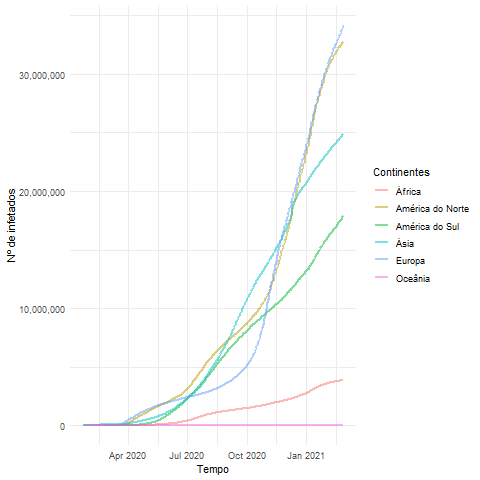
\includegraphics[width=\linewidth]{images/4.1.a.png}
    \caption{Número total de infetados ao longo do tempo, por continente.}
    \label{fig:4.1.a}
\end{figure}

O gráfico \ref{fig:4.1.a} permite verificar um aumento significativo a partir de Abril de 2020,  significativamente a partir de Abril de 2020, nos continentes da Europa e América do Norte, com aumento mais modesto para os restantes continentes, à exceção da Ásia, onde a evolução do número de infetados é geralmente mais conservador, e da Oceânia, onde, devido à sua menor população comparativamente a outros continentes, o número de infetados é negligível quando comparado com os restantes continentes.

De modo a colmatar a negligibilidade do número de infetados na Oceânia e normalizar os resultados de acordo com a população de cada continente, foi produzido um gráfico semelhante ao \ref{fig:4.1.a}, utilizando, em vez do número total de infetados, o número de infetados por milhão de habitantes. Assim, é nos permitido avaliar esta variável sem estarmos expostos a variações devido ao nível populacional de cada continente, o que acontece no gráfico \ref{fig:4.1.a}.

\begin{figure}[h]
    \centering
    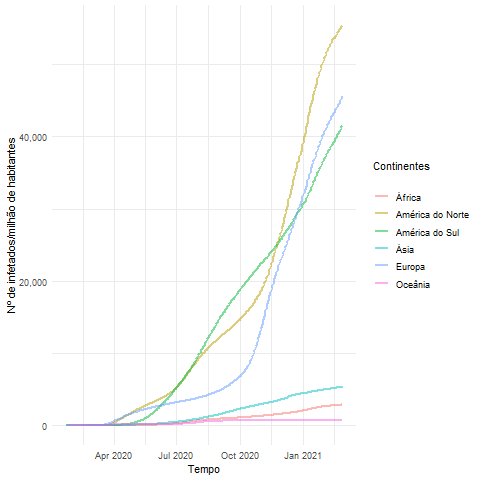
\includegraphics[width=\linewidth]{images/4.1.b.png}
    \caption{Número total de infetados por milhão de habitantes ao longo do tempo, por continente.}
    \label{fig:4.1.b}
\end{figure}

Após análise do gráfico \ref{fig:4.1.b}, podemos verificar de forma mais acentuada que a América do Norte foi o continente com o maior número de infetados por milhão de habitantes. Também é possível verificar uma grande diferença entre dois grupos de continentes. Podemos verificar que a América do Norte, América do Sul e Europa sofreram um aumento de infetados por milhão de habitantes do que a Ásia, África e Oceânia. Esta disparidade pode-se dar devido, por exemplo, ao número de testes efetuados e à disponibilização por partes dos governos de cada país. Assim, numa análise posterior, seria importante avaliar o número de infetados em relação ao número de testes de efetuados, por exemplo.

Em segundo ponto foi feita uma análise sobre a distribuição número de mortes diárias por milhão de habitantes num conjunto de países - Espanha, Itália, Portugal e Reino Unido.

Para este efeito, foi produzido um gráfico de caixa de bigodes, sendo que previamente foram removidos \textit{outliers}, de acordo com a fórmula $x \not\in [Q1 - 1.5 * IQR, Q3 + 1.5 * IQR]$

\begin{figure}[h]
    \centering
    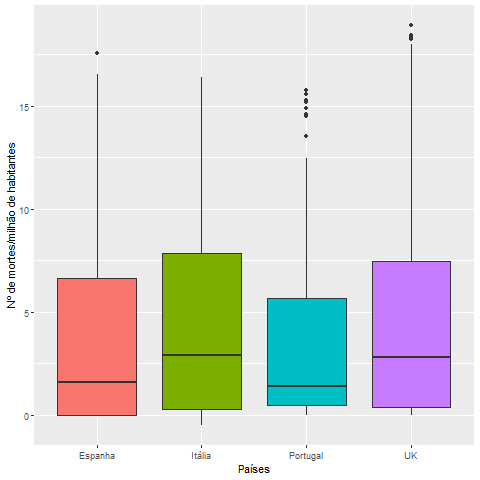
\includegraphics[width=\linewidth]{images/4.1.c.png}
    \caption{Distribuição do número de mortes diárias, para os países Espanha, Itália, Portugal e Reino Unido.}
    \label{fig:4.1.c}
\end{figure}

Podemos verificar que mesmo depois de removidos alguns \textit{outliers}, em Portugal, Espanha e no Reino Unido ainda sobram aqueles que não seguem a condição aplicada. Ainda relativamente ao \textit{outliers}, é possível analisar que o Reino Unido é o país com maiores \textit{outliers} e que a Itália não tem nenhum.

O gráfico ainda mostra que Portugal é o país com menor área de variabilidade dos dados, que os pares Reino Unido/Itália e Portugal/Espanha têm medianas muito semelhantes e que todas estas estão abaixo do centro do retângulo, o que revela o facto de que no quartil superior há uma maior variabilidade de valores.

Em terceiro ponto, foi feita uma análise ao número total de mortos por milhão de habitantes em comparação com o número de testes diários por milhar de habitantes, para um conjunto de países - Albânia, Alemanha, Dinamarca e Rússia.

Para este efeito, foi produzido um gráfico de barras com estas duas variáveis, para cada país em estudo.

\begin{figure}[h]
    \centering
    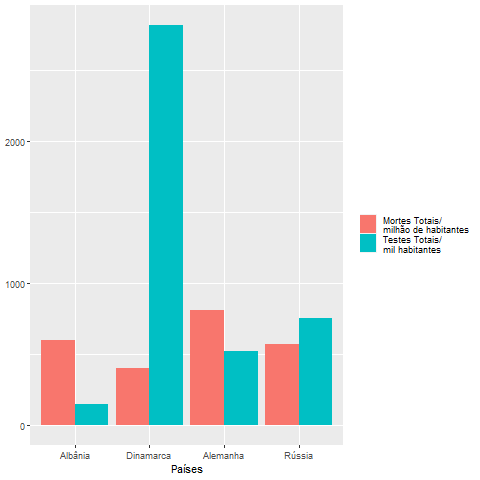
\includegraphics[width=\linewidth]{images/4.1.d.png}
    \caption{Número total de mortes por milhão de habitantes e número de testes diários por milhar de habitantes, para os países Albânia, Alemanha, Dinamarca e Rússia.}
    \label{fig:4.1.d}
\end{figure}

A partir do gráfico \ref{fig:4.1.d} podemos verificar que a Dinamarca lidera no número de testes diários com uma margem considerável, em comparação aos outros três países em análise. Verifica-se também que a Alemanha é o país com maior número de mortes por milhão de habitantes, para o espaço amostral avaliado. Podemos também verificar que, para os países analisados, um maior número de testes por habitante geralmente relaciona-se a um menor número de mortes por habitante. Assim, numa análise posterior, seria interessante alargar esta análise de modo a abranger mais países, com um análise de correlação posterior de modo a validar esta possível relação

Em quarto ponto, foi feita uma análise de modo a obter o país europeu com o maior número de infetados por milhão de habitantes num só dia.

Do processo analítico resultou em que este país é o Vaticano, com aproximadamente $8652.65$ casos por milhão de habitantes (nos dias 12 e 15 de outubro de 2020). Este resultado é expectável, pois este tipo de dado estatístico é suscetível a pequenas populações (o que acontece nos micro-estados, como é o Vaticano). A título de curiosidade, o país europeu não micro-estado que cumpre o predicado referido acima é a Suécia, com $3216.56$ casos por milhão de habitantes no dia 29 de dezembro de 2020.

Em quinto ponto, foi feita uma análise de modo a encontrar o país em que se registou a maior taxa diária de transmissibilidade do COVID-19.

Do processo analítico resultou que o país que cumpre esta estipulação é a Coreia do Sul, com uma taxa de transmissibilidade do vírus de $6.72$ para o dia 22 de fevereiro de 2020.

Em sexto ponto, foi feita uma análise da distribuição do número de mortes diárias por milhão de habitantes por continente.

Como efetuado no segundo ponto, foram removidos os \textit{outliers}, de acordo com a fórmula referida no ponto referido.

Para este efeito foi produzido um gráfico semelhante ao \ref{fig:4.1.b}.

\begin{figure}[h]
    \centering
    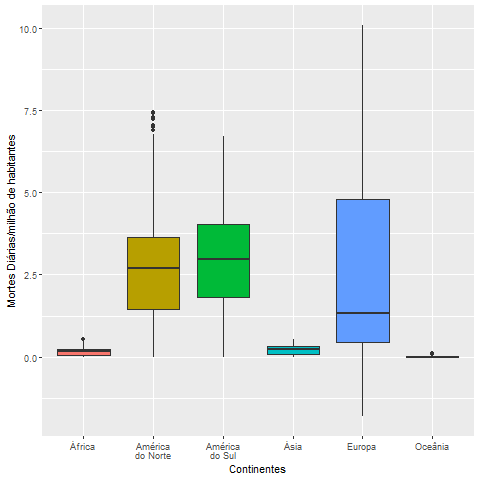
\includegraphics[width=\linewidth]{images/4.1.g.png}
    \caption{Distribuição do número de mortes diárias por milhão de habitantes, por continente.}
    \label{fig:4.1.g}
\end{figure}

Observando o tamanho das "caixas" no gráfico \ref{fig:4.1.g}, é possível observar que África, Ásia e Oceânia têm uma área de variabilidade dos dados muito pequena comparado aos outros continentes. Também conclui-se que a Europa é o continente com maior área de variabilidades dos seis continentes analisados.

Quanto às medianas, verificamos que todas têm valores diferentes, à exceção dos continentes da América do Sul e da América do Norte, que têm medianas com valores próximos. Na Europa, a mediana localiza-se bastante abaixo do centro do retângulo, o que revela que há uma maior variabilidade dos dados acima do valor da mediana.

\subsection{Inferência Estatística}

Primeiramente, foi testado, utilizando uma amostra aleatória de 30 dias, se é possível inferir que a média da taxa de transmissibilidade do vírus no Reino Unido é superior à de Portugal.

Para esse efeito, utilizamos um \textit{$t$-Test} emparelhado, em que $H_{0}$ é a homogeneidade das médias entre as duas amostras e $H_{1}$ é a superioridade da média da amostra referente ao Reino Unido comparativamente à amostra relacionada a Portugal.

Para efetuar este teste, temos que previamente confirmar o pressuposto da normalidade das amostras em causa. Assim, produzimos um gráfico Q-Q para ambas as amostras, de modo a analisar graficamente a normalidade das amostras.

\begin{figure}[h]
    \centering
    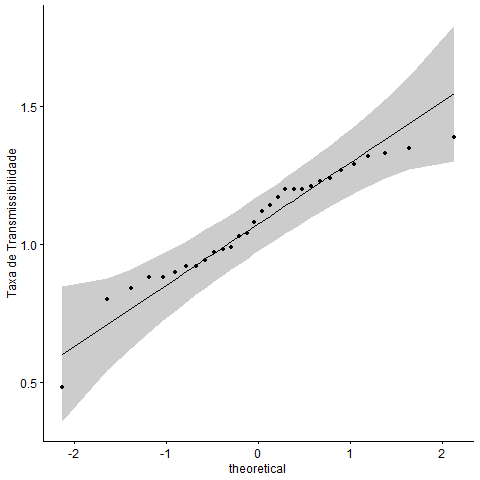
\includegraphics[width=\linewidth]{images/4.2.a_portugal_qqplot.png}
    \caption{Gráfico Q-Q relativo à taxa de transmissibilidade em Portugal.}
    \label{fig:4.2.por}
\end{figure}

\begin{figure}[h]
    \centering
    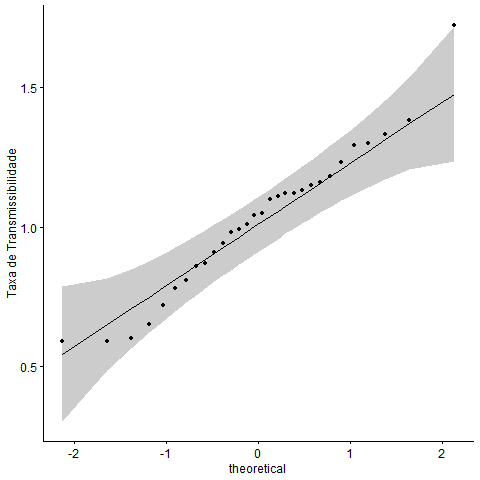
\includegraphics[width=\linewidth]{images/4.2.a_reino_unido_qqplot.png}
    \caption{Gráfico Q-Q relativo à taxa de transmissibilidade no Reino Unido.}
    \label{fig:4.2.uk}
\end{figure}

Ao analisar estes gráficos podemos verificar que ambos são relativamente normais. De notar a existência de um \textit{outlier} nos dados do Reino Unido. Para garantir a normalidade, foi também utilizado o teste de \textit{Shapiro}, em que o $H_{0}$ é a normalidade da dados, sendo que o $H_{1}$ é a não normalidade dos dados. Para este teste assumiu-se um $\alpha$ de $0.05$.

Para Portugal, o teste de \textit{Shapiro} devolveu um \textit{p-value} de $0.13$.

Para o Reino Unido, o teste de \textit{Shapiro} devolveu um \textit{p-value} de $0.46$.

Ambos os \textit{p-value} obtidos encontra-se acima do $\alpha$ definido, o que nos leva a aceitar a hipótese nula e inferir que ambas as amostras provém de uma população normalmente distribuída.


\printbibliography
\end{document}
